\quest{9.1.3}

\partQuest{a}
\begin{description}
    \item[Caso 1] $\delta \ge n$. Não pode ocorrer porque $G$ é simples.

    \item[Caso 2] $\delta = n -1$. Então $G$ é completo e temos que $\kappa = n
    - 1 = \delta$.

    \item[Caso 3] $\delta = n - 2$. Seja $v$ um vértice de $G$ com $d(v) =
    \delta$. Porque $\delta = n - 2$, existe um vértice $u \in V(G)$ não
    adjacente a $v$. Nesse caso, do Teorema 9.2 temos que $\kappa(G) =
    \min\{p(x,y): \,x,y \in V(G), \,x \ne y \, \text{e} \, xy \not \in E(G)\}$.
    Queremos agora determinar $\min \{p(u,v)\}$. Porque $u$ e $v$ não são
    adjacentes e $d(u) \ge \delta$, $u$ deve ser vizinho de todos os vizinhos
    de $v$, o que implica na existência de $n-2$ caminhos internamente
    disjuntos entre $u$ e $v$ através dos seus vizinhos. Portanto, $p(u,v) = n
    - 2 = \delta$ e $\kappa = \delta$.
\end{description}
\fimprova

\partQuest{b}
Seja $G$ o grafo simples com $n$ vértices, $n \ge 4$, tal que $G$ contenha o
grafo completo $K_{n-3}$ como subgrafo e três vértices isolados $v$, $x$ e $y$.
O vértice $v$ será vizinho de todos os vértices do subgrafo $K_{n-3}$. Desse
modo, no subgrafo induzido $G[V(K_{n-3}) \cup \{v\}]$, $\delta = n - 3$. Agora
os vértices $x$ e $y$ serão adjacentes e terão como vizinhos os mesmos $n-4$
vértices do subgrafo $K_{n-3}$ (veja Figura ~\ref{fig:grafokappa}).

\begin{figure}[htb]
    \centering
    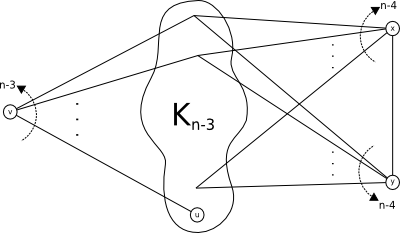
\includegraphics[height=5cm, width=8.6cm]{figuras/graph_q913}
    \caption{Construção do grafo simples $G$ com $\delta = n - 3$ e $\kappa <
    \delta$.}
    \label{fig:grafokappa}
\end{figure}

Note que, porque não inserimos arestas paralelas nem \emph{loops}, $G$ é
simples, possui $n$ vértices e $\delta = n - 3$. Resta mostrar que $\kappa(G) <
\delta$. Como $G$ possui pelo menos um par de vértices não adjacentes, sabemos
do Teorema de Menger que $\kappa$ é igual ao corte mínimo desconectando
qualquer um desses pares. Pelo modo como $G$ foi construído, há um vértice $u
\in V(K_{n-3})$ adjacente a $v$ mas não adjacente nem a $x$ nem a $y$.
Portanto, um corte separando $v$ e $x$ ou $v$ e $y$ deve conter no máximo $n -
4$ vértices do subgrafo $K_{n-3}$. Concluímos que $\kappa(G) \le n - 4 < n - 3
= \delta$.
\fimprova

